% ----------------------------------------------------------
\chapter{Introdução}
% ----------------------------------------------------------

A profícua evolução do processamento computacional proporcionou avanços importantes em diversas áreas do conhecimento humano, como o \textit{design} de fármacos, o planejamento sintético e a ciência de materiais, com alto potencial de aplicabilidade. Essa tendência foi observada por Gordon E. Moore \autocite{Mack2011, Shalf2020}, químico estadunidense 
cofundador da \href{https://www.intel.com/content/www/us/en/company-overview/company-overview.html}{\textit{Intel Corporation}}. A partir dele, foi cunhada uma expressão para designar o aumento bianual de 100\% no número de transistores dos chips microprocessadores, pelo mesmo custo. Isso possibilita, de maneira crescente, a implementação de ferramentas capazes de acessar - seja por meio de cálculos de estrutura eletrônica, 
simulações, ou predições - propriedades que não podem ser obtidas experimentalmente de forma direta. Isto é, uma vez que a química é uma área de difícil abstração por ser acessada na escala quântica da matéria, os computadores ocupam um lugar de destaque no estudo fenomenológico a nível macroscópico \autocite{Allouche2010, Rayan2017}.

Nesse sentido, existe uma pungente necessidade de criar novas abordagens de compreensão da química através da visualização molecular tridimensional, que por vezes faz-se mais efetiva para criar modelos mentais do que o uso de esboços bidimensionais. Importante delimitar que o termo modelagem, aqui, refere-se a um procedimento visual de interação entre a realidade e a teoria a partir de um modelo: filosófico, mecânico ou computacional \autocite{Snyder2021}, cada qual com sua respectiva aproximação. Os fenômenos físicos envolvendo os núcleos dos átomos e seus elétrons são problemas dinâmicos, de múltiplos corpos, que não têm uma solução fechada, pois sistemas quânticos possuem alta complexidade e nem sempre é possível reproduzir de forma analítica os resultados experimentais de interesse.

Esse foi exatamente o processo empenhado ao longo da história da química orgânica: estudar as relações entre as propriedades químicas e a informação estrutural retida por meio de uma compreensão preditiva embasada teoricamente. Indubitavelmente, a aromaticidade desponta nesse sentido como uma das características mais importantes das moléculas, auxiliando na interpretação de dados de reatividade, por exemplo, uma vez que compostos aromáticos apresentam uma preferência pela substituição ao invés da adição, para reter seus elétrons $\pi$ nas reações químicas. Isso foi abordado primeiramente por Roald Hoffmann \autocite{Hoffmann2014}, e desde então tornou-se uma discussão exaustiva dentro da química, sendo desenvolvidos métodos cada vez mais acurados para determinar a geometria molecular e, portanto, suas informações estruturais, como já evidenciado.

Nesse interím, encontrar uma definição de aromaticidade que seja curta, formal e inequívoca é um desafio. Para dirimir tal dificuldade, é possível construir um conjunto de propriedades observadas em compostos que coincidem ao exibir o mesmo caráter aromático, mas de forma multidimensional. Classicamente, a aromaticidade pode ser definida pelo aumento da estabilidade termodinâmica de compostos cíclicos $\pi$-conjugados quando comparados aos seus análogos cujos elétrons são localizados.

Desse modo, é possível comprovar tal tendência avaliando a entalpia envolvida na hidrogenação ($\Delta H^\circ$) de um alceno catalisada por paládio. Tal processo é sempre exotérmico, isto é, libera uma certa quantidade de calor. Por exemplo, se analisarmos a reação de um cicloexeno (\autoref{fig:1}), o valor numérico do $\Delta H^\circ$ será -28,6 kcal/mol (\autoref{fig:2}). 

%% TODO: adicionar imagem sobre estabilização termodinâmica de compostos aromáticos

\begin{figure}[htb]
	\caption{\label{fig:1} Calores de hidrogenação relativos aos hidrocarbonetos cíclicos. Em vermelho, são mostradas as energias de estabilização aromática de cada um dos compostos.}
	\begin{center}
		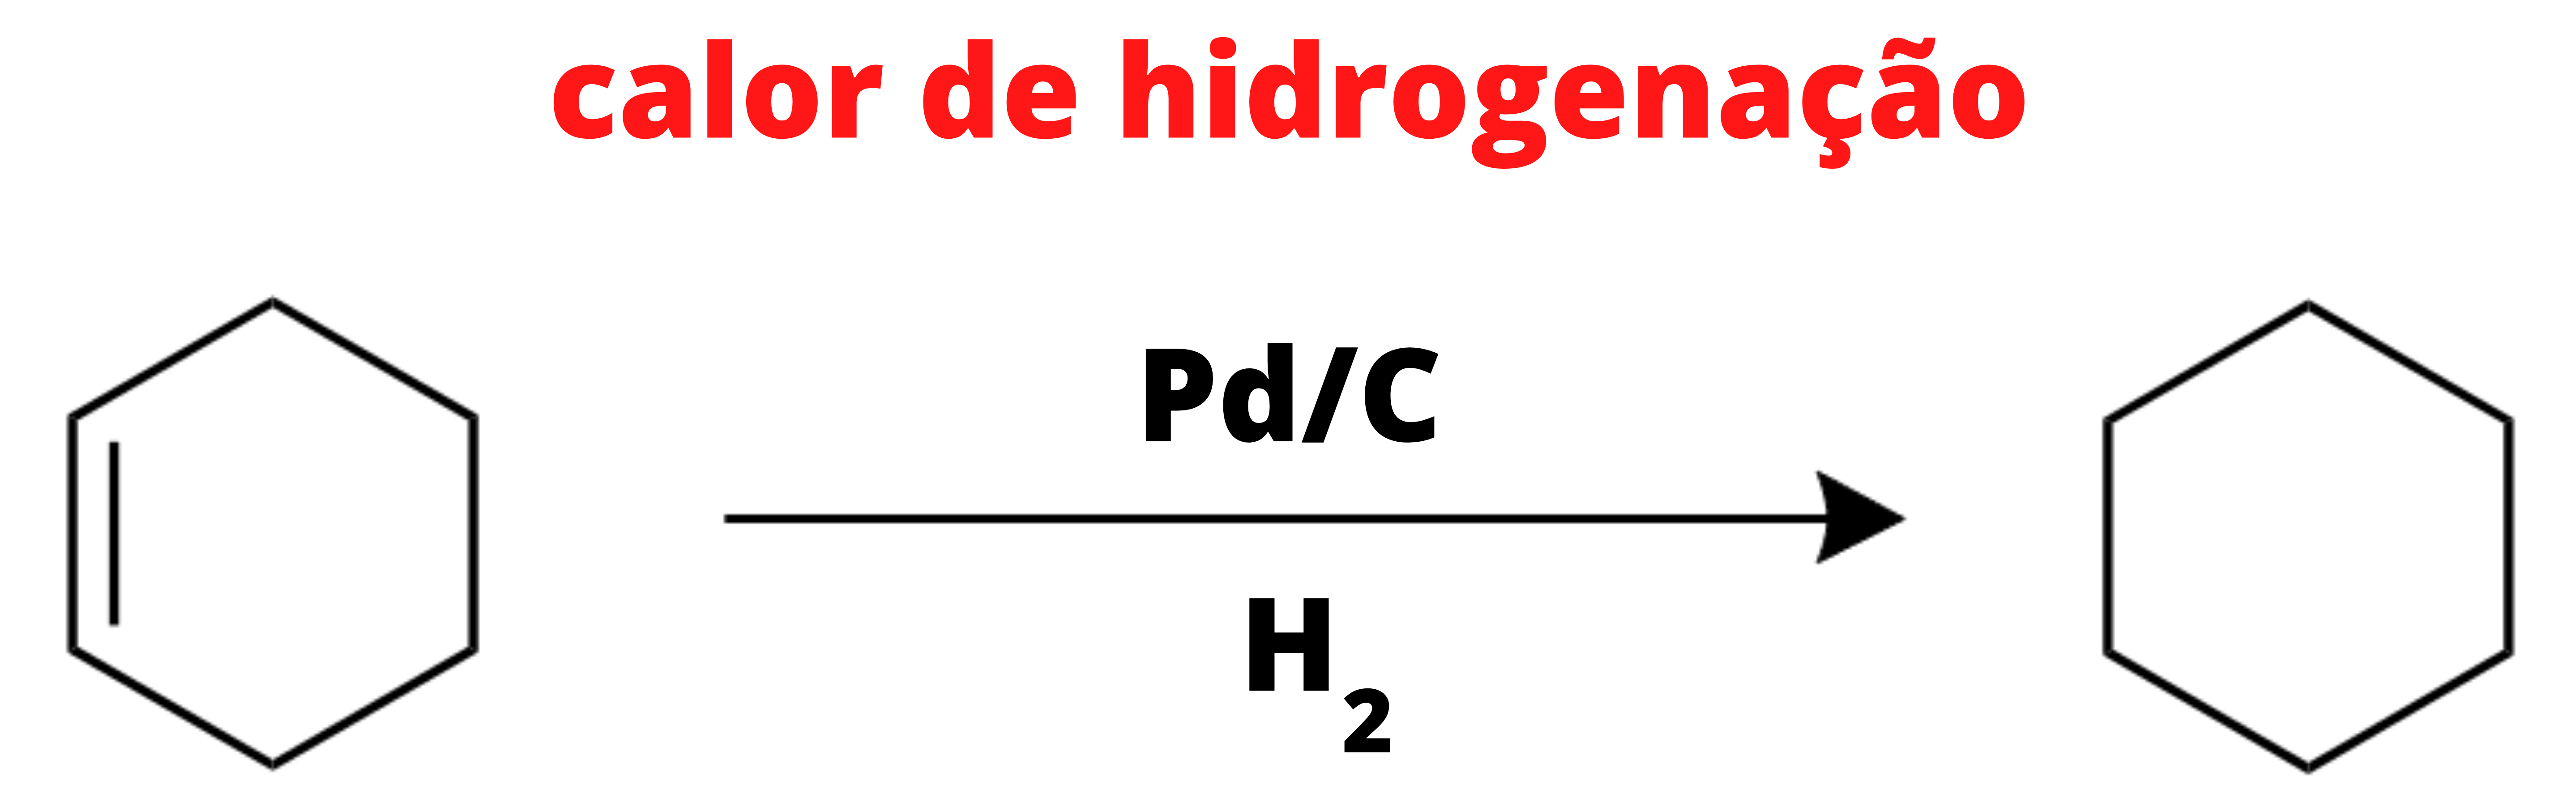
\includegraphics[width=0.5\textwidth]{images/fig1.png}
	\end{center}
	\fonte{Autor(a)}
\end{figure}

Como essa medida é aditiva, se analisarmos o caso do 1,4-cicloexadieno, que possui duas ligações duplas não conjugadas, o calor envolvido no processo será o dobro do que foi observado na situação anterior, isto é, cerca de 56 kcal/mol. No entanto, o isômero conjugado (1,3-cicloexadieno), quando hidrogenado sob as mesmas condições, libera 52,2 kcal/mol (\autoref{fig:2}). A diferença de 3,8 kcal/mol é então chamada de energia de ressonância.

Quando o anel possui três ligações duplas, como na hipótese de um cicloexatrieno, o valor numérico esperado para a entalpia de hidrogenação seria de 85,8 kcal/mol (o triplo do exemplo inicial). Porém, quando essa reação é realizada em condições normais (Pd/C, temperatura ambiente, 1 atm de H$_2$), nada acontece porque o reagente é inerte. Se a pressão for gradualmente aumentada, o cicloexatrieno permanece intacto. Finalmente, submetendo o meio a uma situação drástica (temperatura de 180-220$^\circ$C e 25-30 atmosferas de gás hidrogênio), o reagente hipotético, enfim, gera um cicloexano. Ao medir o calor liberado, o resultado é surpreendente, uma vez que a entalpia obtida é 49,8 kcal/mol, ou seja, 36 kcal/mol abaixo do resultado que era previsto (\autoref{fig:2}). Acontece que o substrato do meio reacional em questão é o benzeno, uma estrutura totalmente conjugada e, por conseguinte, estabilizada pela sobreposição dos orbitais p \autocite{Shaabani2008, Xu2021}. Em função disso, torna-se indispensável a análise comparativa das energias associadas aos orbitais moleculares (\gls{MOs}), uma vez que o caráter covalente da ligação aumenta, e a diferença de energia entre os orbitais de fronteira diminui quando comparamos as espécies aromáticas e seus análogos sem conjugação.

\begin{figure}[htb]
	\caption{\label{fig:2} Calores de hidrogenação relativos aos hidrocarbonetos cíclicos. Em vermelho, são mostradas as energias de estabilização aromática de cada um dos compostos.}
	\begin{center}
		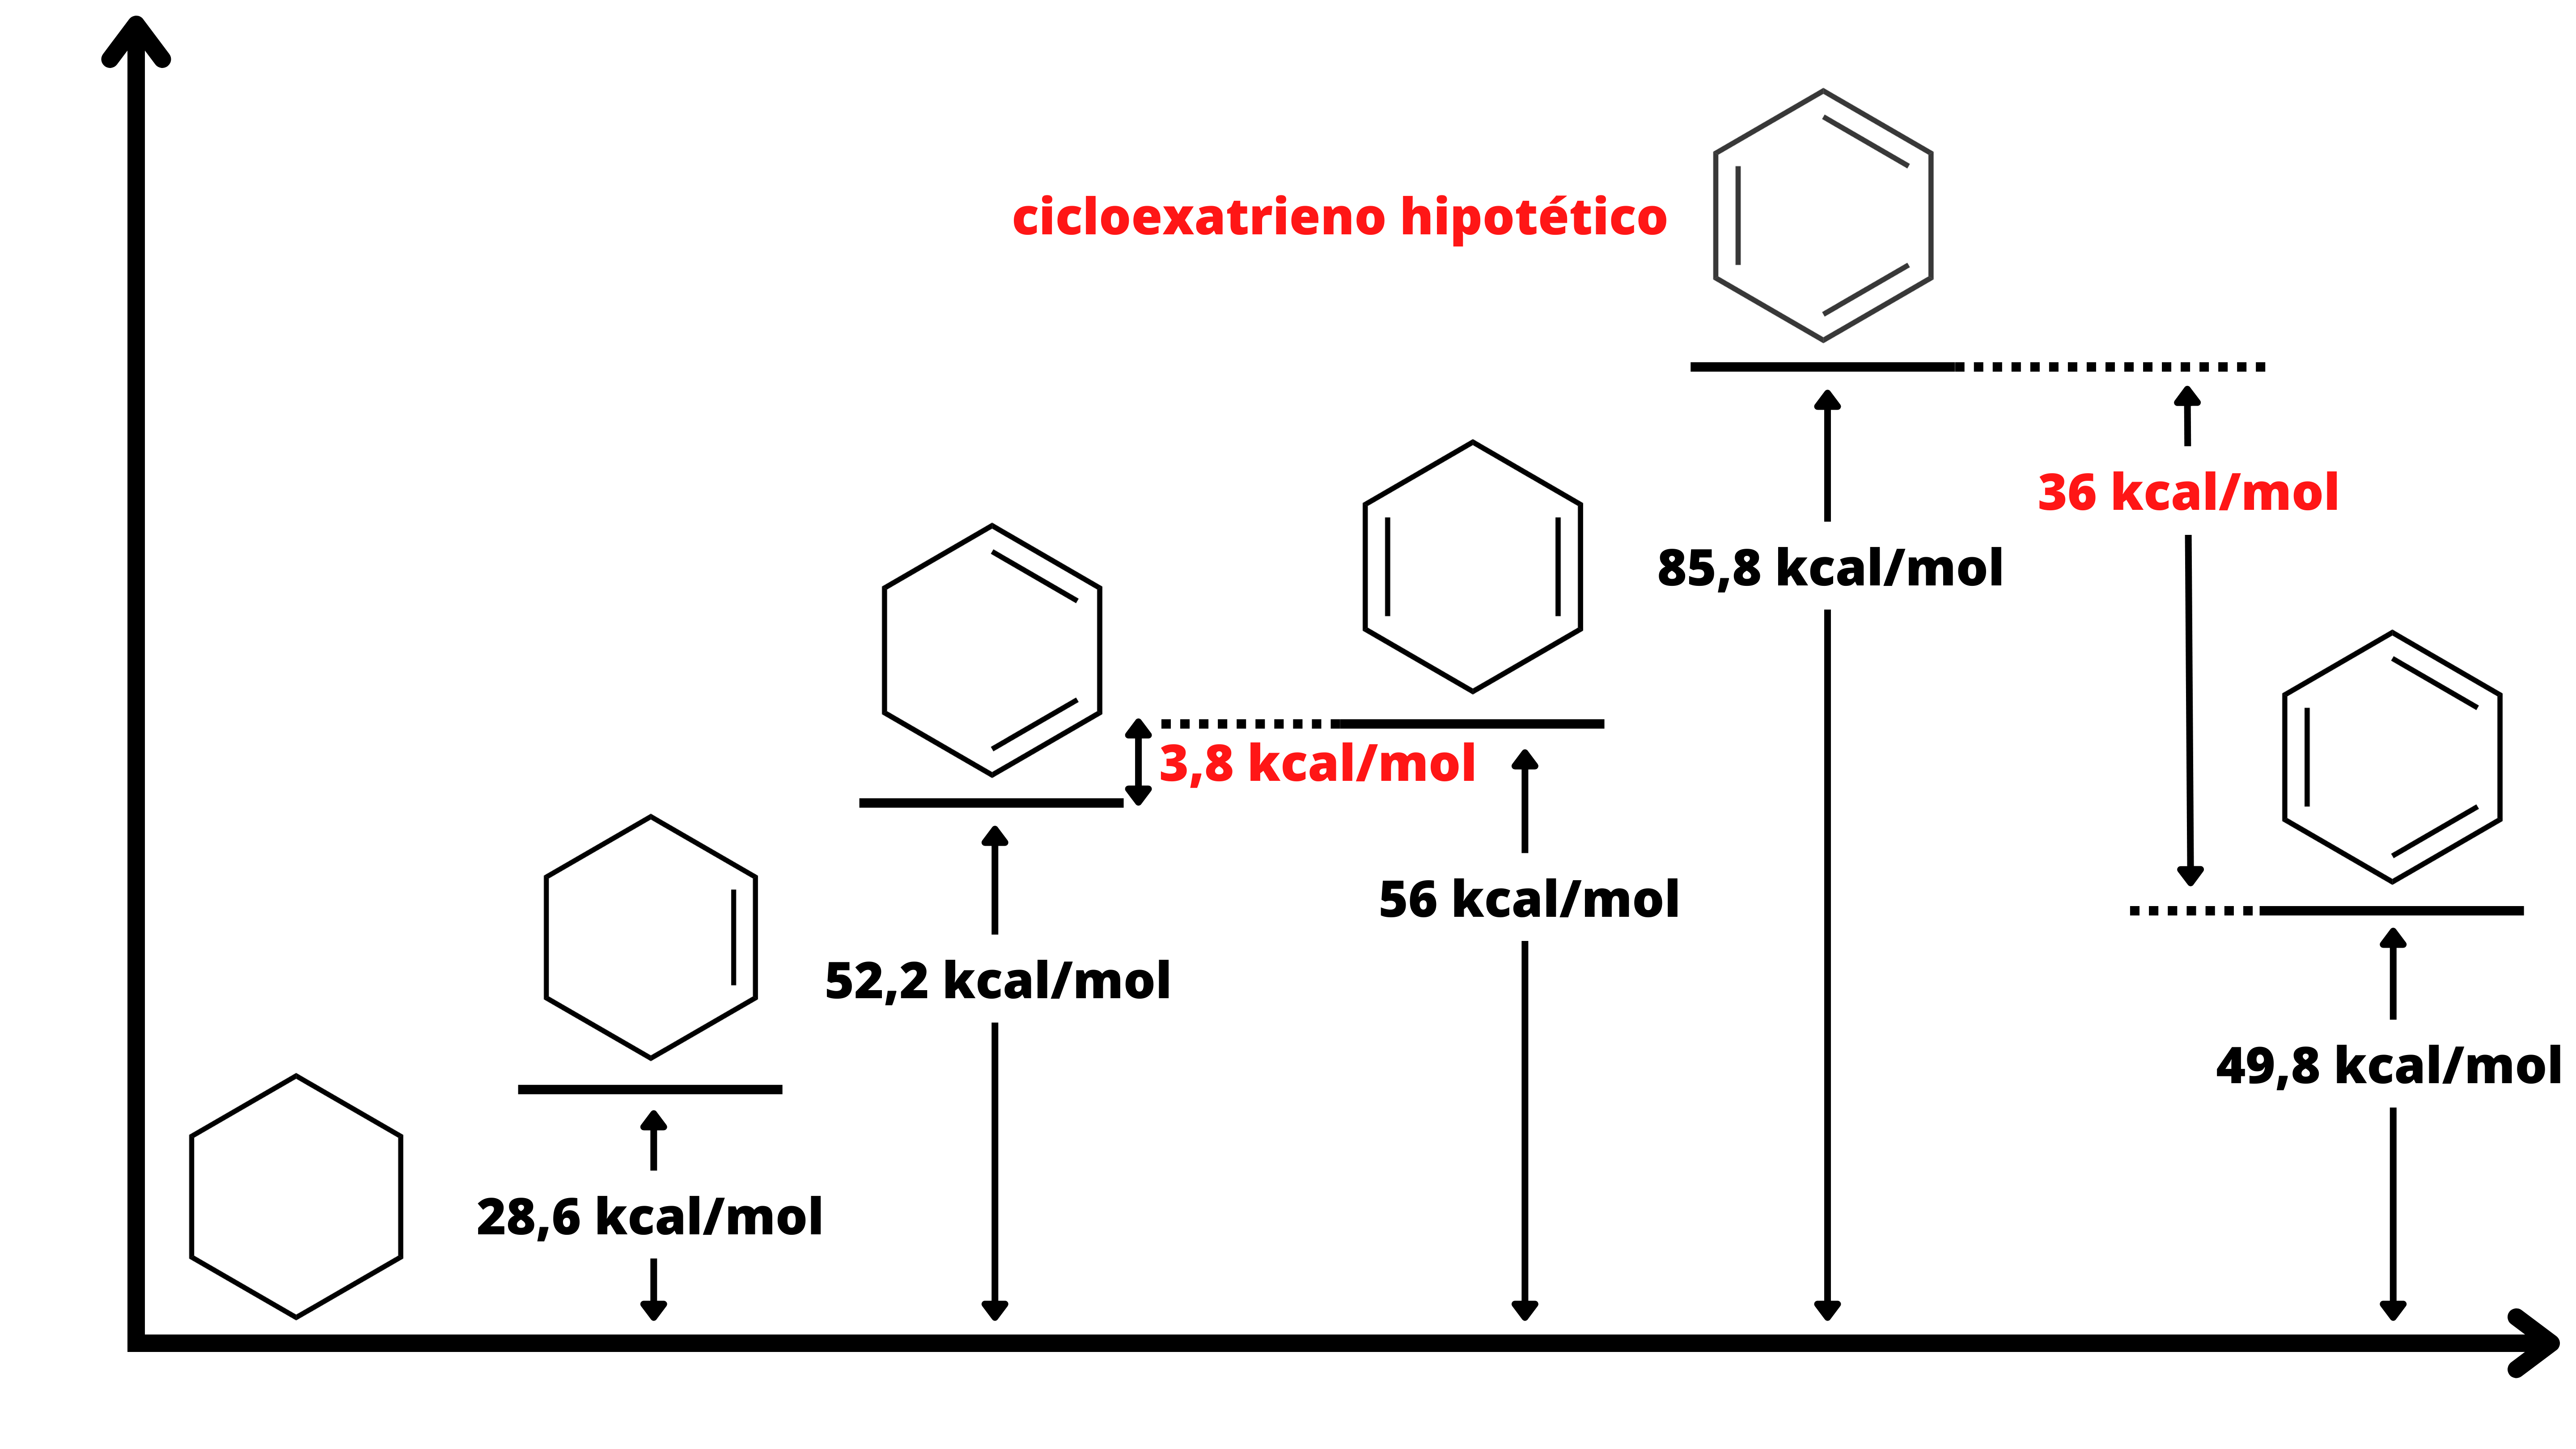
\includegraphics[width=1.0\textwidth]{images/fig2.png}
	\end{center}
	\fonte{Autor(a)}
\end{figure}

%% TODO: falar dos orbitais moleculares de fronteira na aromaticidade.

Como o conceito de aromaticidade é multidimensional, um problema recorrente nessas representações é que um dado critério utilizado para classificar esses compostos não pode, em geral, ser aplicado de maneira consistente. Em muitos casos, encontrar um ponto de referência apropriado é problemático. Por exemplo, os valores de energia de estabilização aromática dependem profundamente dos sistemas de referência em reações virtuais, uma vez que é praticamente impossível deduzir diferenças na aromaticidade de acordo com tendências de reatividade, a menos que sejam consideradas séries de reações estruturalmente similares, a citar, os hidrocarbonetos benzenoides \autocite{Ciesielski2009, Krygowski2014}. Nesse sentido, índices baseados na geometria molecular, tal como \gls{HOMA} \autocite{Kruszewski1972}, também são relativos à escala. 

% Ou seja, a computação gráfica auxilia na manipulação/representação direta dos objetos de estudo químico, sendo eles: átomos, moléculas (leia-se quaisquer agregados atômicos, independentemente da origem de suas interações) ou partes delas. Como esses são elementos de difícil abstração, uma vez que 

% Em tal seguimento, um dos avanços mais importantes é a aplicação da teoria de grafos à notação química e aos sistemas de busca de subestruturas e cálculos de propriedades, como a aromaticidade, que é muito sensível à geometria do sistema $\pi$, pois descreve as moléculas estabilizadas energeticamente pela deslocalização de elétrons móveis em ciclos (geometrias fechadas). Tal temática é extremamente explorada por trabalhos que vem sendo somados desde a primeira citação de Hoffmann na literatura, em 1855. Por exemplo, com uma busca sobre os termos aromático/aromaticidade no \textit{\href{https://scholar.google.com.br/scholar?hl=pt-BR&as_sdt=0\%2C5&as_ylo=2016&as_yhi=2022&q=aromatic&btnG=}{Google Scholar}} no período de 2016 a 2022, foram encontrados mais de 380 trabalhos/dia publicados, sendo a maioria destes na área de Química, uma vez que, entre os compostos carbocíclicos, destacam-se os derivados aromáticos, cuja estabilidade e reatividade dependem do caráter de deslocalização eletrônica. Para tais sistemas, é possível utilizar a equalização dos comprimentos de ligação como principal critério geométrico de análise quantitativa.


O presente trabalho pretende, fundamentado nesse conjunto de informações, relacionar as propriedades extraídas das representações moleculares a partir da computação gráfica, produzindo uma interface para manipular esses compostos de forma facilitada e didática. % Assim, usuário será capaz de calcular os parâmetros geométricos de aromaticidade, um conceito explorado de forma superficial e pouco visual dentro das salas de aula. 

Uma vez que as dificuldades de compreensão por parte dos graduandos em relação aos conceitos e fenômenos originam-se na forma com que são apresentados \autocite{Cunha2018}, a ferramenta proposta poderá ser difundida para uso didático-pedagógico, podendo ser utilizada por discentes e docentes durante as aulas no sentido de demonstrar os modelos de classificação e a multidimensionalidade da aromaticidade, facilitando o entendimento.

% ----------------------------------------------------------
\section{Recomendações de uso}
% ----------------------------------------------------------

Este \emph{template} foi elaborado para se compilado em \LaTeX utilizando \abnTeX.  Todas as configurações de diferenciação gráfica nas divisões de seção e subseção seguem a  norma NBR 6027/2012 automaticamente. 

Uma nota de rodapé, já tem seu estilo automático com o comando \texttt{$\backslash$footnote}\footnote{As notas de rodapé possuem fonte tamanho 10. O alinhamento das linhas da nota de rodapé deve ser abaixo da primeira letra da primeira palavra da nota de modo dar destaque ao expoente.}.


% ----------------------------------------------------------
\chapter{Objetivos}
% ----------------------------------------------------------

% ----------------------------------------------------------
\section{Objetivo Geral}
% ----------------------------------------------------------

 Desenvolver um \textit{software} de interação gráfica capaz de representar a molécula tridimensionalmente através da leitura de dados de coordenadas cartesianas atômicas e assim retornar parâmetros de aromaticidade segundo a metodologia definida pelo usuário. Poderá, portanto, ser utilizado como uma ferramenta de pós-processamento para o cálculo de propriedades eletrônicas. Além disso, também pretende-se implementar métodos semiempíricos de baixo custo computacional (Hueckel e Hueckel estendido) para auxiliar na avaliação e representação dos orbitais atômicos e moleculares.

% ----------------------------------------------------------
\section{Objetivos Específicos}
% ----------------------------------------------------------

\begin{itemize}
    %\item Realizar pré-otimizações de geometria utilizando métodos semi-empíricos e \textcolor{red}{realizando leituras de estruturas obtidas por outros métodos através de outros \textit{softwares}; complementar};
    
    \item Utilizar métodos semiempíricos para avaliar orbitais atômicos e moleculares.
    
    \item Automatizar a leitura de arquivos de saída \textit{outputs} \textit{logfiles} de cálculos de estrutura eletrônica molecular visando extrair dados geométricos para determinar critérios de aromaticidade geométricos em sistemas orgânicos, através de uma interface gráfica.

    \item Utilizar a teoria de grafos para implementar a determinação dos índices HOMA, EN, e GEO; 
    
    \item Realizar \textit{benchmark} dos resultados obtidos com estruturas já reportadas na literatura para fins de  validação e comparação do tempo de computação na metodologia aplicada.
\end{itemize}